\documentclass[a4paper, oneside, 11pt]{report}
\usepackage[a4paper, vmargin=1.0cm, top=0.5cm, bottom=2.0cm, headsep=1.0cm, nofoot ]{geometry}
\usepackage[utf8]{inputenc}      			% kodowanie literek
\usepackage[polish]{babel}				% reguły dla języka polskiego
\usepackage[OT4]{fontenc}				% ładne czcionki w PDFie
\usepackage{polski}					% polski
\usepackage{indentfirst} 				% wcięcia pierwszego akapitu
\usepackage{anysize}
% \usepackage{wrapfig} 					% oblewanie rysunków tekstem
\usepackage[pdftex]{graphicx} 				% dołączanie obrazków - tryb pdftex

\makeindex

\title{Projekt Service Desk}
\author{Piotr Kalański, Adrian Wiśniewski}



\selectlanguage{polish} 		% wybierz polski

\begin{document}

\maketitle

\tableofcontents

\pagestyle{headings}

\chapter{Słownik}

\begin{description}
 \item[Usługa] (Service).
 \item[Incydent] Zdarzenie, które nie jest cześcią standardowej pracy, które może doprowadzić do zakłucenia lub obniżenia jakości usługi.
 \item[Problem] Przyczyna wystąpienia jednego lub więcej incydentów.
 \item[RFC] Request For Change - żądanie wprowadzenia zmiany np. związanej ze sprzętem, oprogramowaniem itp.
 \item[CI] Configuration Item - element konfiguracji, może składać się z innych CI.
 \item[PIR] Post Implementation Review - weryfikacja wprowadzonej zmiany po implementacji. Obejmuje sprawdzenie reakcji klienta na zmianę i czy nie nastąpiły niespodziewane efekty uboczne.
 \item[Change Model] szablon postępowania z regularnymi zmianami
 \item[Znany bład] (Known error) - incydent lub błąd, dla którego jest znana przyczyna oraz dla którego znaleziono tymczasowe rozwiązanie lub stałą alternatywę.
 \item[KEDB] Known Error Database
 \item[DSL] Definitive Software Library - zbiór wszystkich autoryzowanych wersji wszystich elementów oprogramowania (software CI) i kodów źródłowych
 \item[DHS] Definitive Hardware Store - zbiór wszystkich zapasowych elementów sprzętu komputerowego ( hardware CI )
 \item[Wydanie] (Release) - kolekcja autoryzowanych zmian w usłudze IT. Jest zdefiniowane przez RFC implementujące te zmiany.
\end{description}

\chapter{Wymagania funkcjonalne}

\begin{description}
 \item[F.IM.0] Zarządzanie incydentami (Incident Management).
  \begin{description}
   \item[F.IM.1] Dodawanie incydentów.
   \item[F.IM.2] Klasyfikacja incydentów.
   \item[F.IM.3] Eskalacja incydentów do grup roboczych.
   \item[F.IM.4] Zamykanie incydentów.
   \item[F.IM.5] Nadawanie priorytetów incydentom.
   \item[F.IM.6] Status incydentu.
   \item[F.IM.7] Powiązanie incydentu z CI.
   \item[F.IM.8] Automatyczna eskalacja po przekroczeniu terminu.
   \item[F.IM.9] Wyszukiwanie incydentów.
   \item[F.IM.10] Raportowanie.
    \begin{description}
      \item[F.IM.10.1] Raport o liczbie zrealizowanych incydentów danej kategorii w danym okresie czasu.
      \item[F.IM.10.2] Raport o liczbie zrealizowanych incydentów przez daną grupę wsparcia.
      \item[F.IM.10.3] Raport o liczbie zrealizowanych incydentów przez danego pracownika.
      \item[F.IM.10.4] Raport o liczbie incydentów o danym statusie w danym orkesie czasu.
    \end{description}
    \item[F.IM.11] Dodawanie uwag do incydentów.
    \item[F.IM.12] Przeglądanie historii konkretnego incydentu.
    \item[F.IM.G] Zarządzanie grupami wsparcia.
      \begin{description}
        \item[F.IM.G.1] Dodawanie członków do grupy wsparcia.
        \item[F.IM.G.2] Usuwanie członków z grup wsparcia.
        \item[F.IM.G.3] Dodawanie grup wsparcia.
        \item[F.IM.G.4] Przypisywanie grup wsparcia do kategorii incydentów.
      \end{description}
    \item[F.IM.13] Powiadamianie drogą mailową o zmianie statusu incydentu zainteresowanych osób.
  \end{description}
 \item[F.PM.0] Zarządzanie problemami (Problem Management).
  \begin{description}
   \item[F.PM.1] Identyfikacja i zapisywanie problemów.
   \item[F.PM.2] Klasyfikacja problemów.
   \item[F.PM.3] Dodawanie błędów do KEDB.
   \item[F.PM.4] Wyszukiwanie problemów.
   \item[F.PM.5] Wyszukiwanie znanych błędów.
   \item[F.PM.6] Wycena błędów.
   \item[F.PM.7] Zamykanie błędów.
   \item[F.PM.R] Dodawanie recenzji do problemów.
  \end{description}
 \item[F.CM.0] Zarządzanie konfiguracją (Configuration Management).
  \begin{description}
   \item[F.CM.1] Zarządzanie typami CI.
   \item[F.CM.2] Historia CI.
   \item[F.CM.3] Zarządzanie typami atrybutów CI.
   \item[F.CM.4] Zarządzanie atrubytami CI.
   \item[F.CM.5] Zarządzanie typami związków.
   \item[F.CM.6] Zarządzanie rolami w związkach
   \item[F.CM.7] Zarządzanie związkami między CI.
   \item[F.CM.8] Dodawanie CI.
   \item[F.CM.9] Wyszukiwanie CI.
   \item[F.CM.10] Zmiany CI.
   \item[F.CM.11] Zarządzanie wariantami CI.
   \item[F.CM.12] Wyszukiwanie poprzednich wersji CI.
   \item[F.CM.13] Zastępowanie aktualnej wersji CI wersją z przeszłości.
  \end{description}
 \item[F.ChM.0] Zarządzanie zmianami (Change Management).
 \begin{description}
   \item[F.ChM.1] Wprowadzanie żądań zmian (RFC)
   \item[F.ChM.C] Ustawianie priorytetu i kategorii zmian
    \begin{description}
     \item[F.ChM.C.1] W szczególności oznaczenie żądania jako pilne (Urgent)
    \end{description}
   \item[F.ChM.2] Filtrowanie żądań zmian
   \item[F.ChM.3] Wspieranie oceny zmian
   \item[F.ChM.4] Wspieranie autoryzacji zmian
   \item[F.ChM.5] Utrzymywanie bazy predefiniowanych procedur wdrażania zmian (Change Model)
   \item[F.ChM.6] Wsparcie dla procedury wykonywania zwykłych zmian
   \item[F.ChM.7] Wsparcie dla procedury wykonywania zmian pilnych
   \item[F.ChM.8] Zatwierdzanie wykonania zmian
   \item[F.ChM.9] Weryfikacja zmiany po implementacji (PIR)
  \end{description}
 \item[F.RM.0] Zarządzanie wydaniami (Release Management).
  \begin{description}
   \item[F.RM.1] Wsparcie dla planowania wydań
   \item[F.RM.2] Wsparcie dla polityki wydawniczej
   \item[F.RM.3] Gromadzenie wymaganego oprogramowania i sprzętu z centralnej bazy konfiguracji (CMDB)
   \item[F.RM.4] Wsparcie dla testowania i akceptacji wydania
   \item[F.RM.5] Wsparcie dla przeprowadzania wydań (rollout)
   \item[F.RM.6] Wsparcie dla wdrożenia wydania
   \item[F.RM.7] Planowanie szkoleń związanych z wydawanym produktem lub usługą
   \item[F.RM.8] Wsparcie dla komunikacji z klientem
   \item[F.RM.DSL] Zarządzanie biblioteką oprogramowania (DSL)
    \begin{description}
     \item[F.ChM.DSL.1] Zarządzanie licencjami
	 \item[F.ChM.DSL.2] Wspracie dla audytów oprogramowania
    \end{description}
   \item[F.RM.DHS] Zarządzanie magazynem sprzętu (DHS)
  \end{description}
\end{description}

\chapter{Przypadki użycia}
\section{Aktorzy}

\begin{description}
 \item[Pracownik] Osoba, która może zgłosić incydent lub RFC.
 \item[Członek grupy wsparcia] Osoba odpowiedzialna za rozwiązanie problemu.
 \item[Menager problemów] Osoba zarządzająca członkami grup wsparcia.
\end{description}

\chapter{Projekt bazy danych}

\section{Fragment bazy danych związany z incydentami}

\subsection{INCIDENTS}

Tabela zawierająca informacje o incydentach.

\paragraph{INCIDENT\_ID} id incydentu nadawane za pomocą sekwencji
\paragraph{IMPACT} miara określająca wpływ incydentu na biznes
\paragraph{URGENCY} miara określająca pilność incydentu
\paragraph{STATUS\_CODE} kod statusu incydentu
\paragraph{REVIEW} opis czego dotyczy incydent
\paragraph{PRIORITY} priorytet obliczany na podstawie IMPACT oraz URGENCY
\paragraph{AUTHOR} osoba, która dodała ten incydent
\paragraph{CATEGORY\_CODE} kod kategorii do jakiej należy ten incydent
\paragraph{TYPE} typ incydentu: incydent lub service request
\paragraph{CREATION\_DATE} data utworzenia incydentu
\paragraph{CLOSURE\_DATE} data zamknięcia incydentu

\subsection{INCIDENT\_CATEGORIES}

Tabela zawierająca informacje o kategoriach incydentów. Każda kategoria może mieć swoją nadkategorie.

Możliwe kategorie:

\begin{itemize}
 \item Sprzęt
      \begin{itemize}
	\item Stacja robocza
	\item Mainframe
       \end{itemize}
 \item Oprogramowanie
      \begin{itemize}
	\item Arkusz kalkulacyjny
	\item Edytor tekstu
       \end{itemize}
\end{itemize}

\paragraph{CATEGORY\_CODE} Unikalny kod kategorii.
\paragraph{NAME} Nazwa kategorii
\paragraph{PARENT\_CATEGORY} Kategoria nadrzędna.
\paragraph{GROUP\_ID} Id grupy odpowiedzialnej za tą kategorię.

\subsection{INCIDENT\_STATUSES}

Tabela zawierająca informacje o możliwych statusach incydentów: nowy, zaakceptowany, zaszeregowany, przypisany do, w trakcie pracy, zamknięty.

\paragraph{STATUS\_CODE} Unikalny kod statusu.
\paragraph{NAME} Nazwa statusu

\subsection{SUPPORT\_GROUPS}

Tabela zawierająca informacje o grupach wsparcia. Każda grupa składa się z dowolnej liczby pracowników oraz jest odpowiedzialna za incydenty z danej kategorii.

\paragraph{GROUP\_ID} Unikalne id grupy.
\paragraph{NAME} Nazwa grupy.

\subsection{GROUP\_MEMBER}

Tabela zawierająca informacje o członkach grup wsparcia.

\paragraph{GROUP\_ID} Id grupy.
\paragraph{EMPLOYEE\_ID} Id pracownika należącego do grupy.

\subsection{EMPLOYEES}

Tabela zawierająca informacje o pracownikach firmy.

\paragraph{EMPLOYEE\_ID} Unikalne id pracownika.
\paragraph{NAME} Imię pracownika.
\paragraph{SURNAME} Nazwisko pracownika.

\begin{figure}[!ht]
\centering
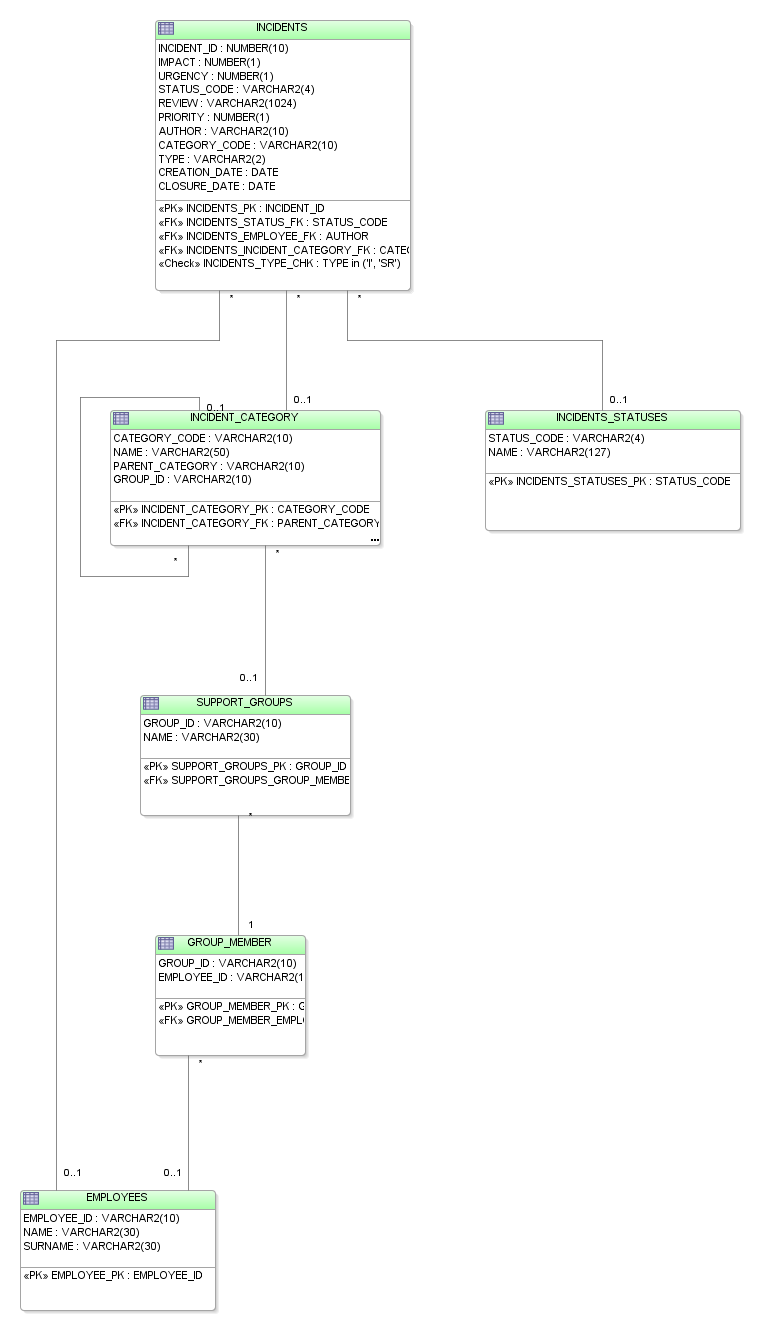
\includegraphics[width=14cm]{incydenty.png}
\caption{Incydenty}
\end{figure}


\section{Fragment bazy danych związany z konfiguracją}

\subsection{CONFIGURATION\_ITEMS}

Tabela zawierająca informacje o posiadanych rzeczach przez firmę, które objęte są zarządzaniu konfiguracją.

\paragraph{ITEM\_ID} Unikalne id
\paragraph{TYPE\_ID} Id typu

\subsection{ITEM\_TYPES}

Tabela zawierająca informacje o typach posiadanych rzeczy.

\paragraph{TYPE\_ID} Unikalne id typu
\paragraph{NAME} Nazwa typu
\paragraph{PARENT\_ID} Nazwa typu nadrzędnego

\subsection{ATTRIBUTE\_ITEM\_TYPE}

Tabela zawierająca informacje o atrybutach przypisanych do konkretnego typu atrybutu.

\paragraph{ATTRIBUTE\_ID} Id atrybutu
\paragraph{TYPE\_ID} Id typu

\subsection{ATTRIBUTE\_TYPES}

Tabela zawierająca informacje o typach atrybutu.

\paragraph{ATTRIBUTE\_ID} Id atrybutu
\paragraph{ATTRIBUTE\_NAME} Nazwa atrybutu

\subsection{ATTRIBUTE\_VALUES}

Tabela zawierająca informacje o wartościach konkretnych rzeczy dla konkretnych atrybutów.

\paragraph{ATTRIBUTE\_ID} Id atrybutu
\paragraph{ITEM\_ID} Id rzeczy
\paragraph{VALUE} Wartość atrybutu

\subsection{RELATIONSHIP\_TYPES}

Tabela zawierająca informacje o typach relacji między rzeczami.

\paragraph{RELATIONSHIP\_TYPE\_ID} Unikalne id związku
\paragraph{NAME} nazwa związku

\subsection{RELATIONSHIP\_ROLES}

Tabela zawierająca informacje o rolach w relacjach.

\paragraph{RELATIONSHIP\_TYPE\_ID} Id typu związku
\paragraph{RELATIONSHIP\_ROLE\_ID} Id roli w związku, np parent, child, is part of
\paragraph{NAME} Nazwa roli

\subsection{RELATIONSHIPS}

Tabela zawierająca informacje o konkretnych relacjach.

\paragraph{RELATIONSHIP\_TYPE\_ID} Id typu związku 
\paragraph{RELATIONSHIP\_ID} Id związku

\subsection{RELATIONSHIP\_ITEM}

Tabela zawierająca informacje o uczestnikach konkretnych relacji.

\paragraph{RELATIONSHIP\_TYPE\_ID} Id typu związku 
\paragraph{RELATIONSHIP\_ROLE\_ID} Id roli w związku
\paragraph{RELATIONSHIP\_ID} Id związku
\paragraph{ITEM\_ID} Id rzeczy

\begin{figure}[!ht]
\centering
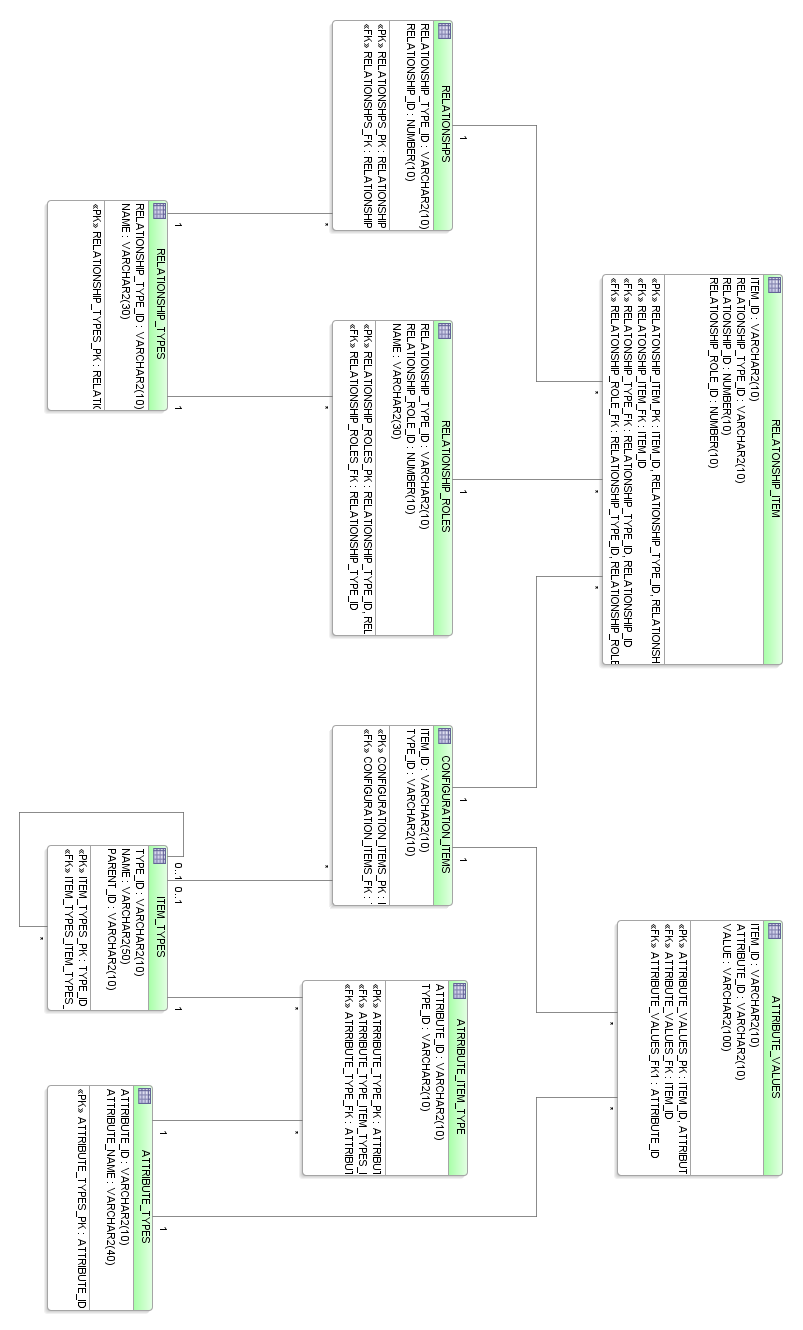
\includegraphics[width=14cm]{ci.png}
\caption{Configuration Items}
\end{figure}


\section{Fragment bazy danych związany z zmianami}

\subsection{CAB}

Tabela zawierajšca informacje o grupach ludzi uczestniczšcych w przeprowadzeniu zmiany.

\paragraph{CAB\_ID} unikalne id
\paragraph{NAME} nazwa

\subsection{CAB\_MEMBER} Tabela zawierajšca informacje o członkach grup uczestniczšcych w przeprowadzeniu zmiany.

\paragraph{RFC\_ID} Id rfc
\paragraph{EMPLOYEE\_ID} Id pracownika
\paragraph{ROLE\_ID} Id roli w tej grupie


\paragraph{CAB\_MEMBER\_ROLES} Tabela zawierajšca informacje o rolach pracowników w grupach CAB

\paragraph{ROLE\_ID} Id roli
\paragraph{NAME} Nazwa roli

\subsection{RFC} Tabela zawierajšca informacje o proponowanych zmianach.

\paragraph{RFC\_ID} Id zmiany
\paragraph{CREATION\_DATE} Data dodania
\paragraph{TYPE\_CODE} Typ zmiany
\paragraph{PRIORITY} Priorytet zmiany
\paragraph{IS\_URGENT} Czy to zmiana pilna
\paragraph{REVIEW} Recenzja zmiany
\paragraph{COST} Szacowany koszt
\paragraph{IMPACT} Miara określająca wpływ zmiany
\paragraph{ESTIMATED\_TIME} Szacowany czas wprowadzenia zmiany
\paragraph{CATEGORY} Kategoria zmiany: minor, significant, major
\paragraph{STATUS\_CODE} Status zmiany: Proponowana, Odrzucona, w trakcie budowy, zamknięta


\subsection{RFC\_STATUSES}  Tabela zawierajšca informacje o możliwych statusach zmian
\paragraph{STATUS\_CODE} Kod statusu
\paragraph{NAME} Nazwa statusu

\subsection{RFC\_TYPES}  Tabela zawierajšca informacje o typach zmian
\paragraph{TYPE\_CODE} Kod typu
\paragraph{NAME} Nazwa typu
\paragraph{PARENT\_CODE} Typ nadrzędny


\begin{figure}[!ht]
\centering
\includegraphics[width=14cm]{change.png}
\caption{Changes}
\end{figure}

\chapter{Technologia wykonania}

System postanowiliśmy wykonać jako aplikację WWW w technologi J2EE z interfejsem użytkownika w postaci przeglądarki. 
Takie rozwiązanie pozwoli na zminimalizowanie kosztów wdrożenia i aktualizacji systemu, a także umożliwi skalowanie 
w zależności od potrzeb. Ponadto pozwoli to na zdalny dostęp do zasobów systemu poza stanowiskiem pracy, co może być 
ważne np. dla kadry menedżerskiej.

Pojednycze komponenty systemu, które będą wymagały przechowywania dużej ilości informacji na stacji roboczej zostaną 
wykonane jako aplikacje okienkowe w technologii Java Swing i będą łączyły się z systemem za pomocą usług sieciowych (Web Services).

\chapter{Wykorzystywane narzędzia}

\section{Oracle Database 10g Express Edition}

Wykorzystana jako relacyjna baza danych.

\section{Apache Tomcat}

Serwer WWW

\section{Spring framework 3.0}

Szkielet do tworzenia aplikacji w języku Java dla platformy Java EE/J2EE.

\section{SpringSource Tool Suite}

Wykorzystany jako IDE do stworzenia aplikacji w Spring framework.

\section{Netbeans}

Wykorzystany jako IDE do stworzenia aplikacji okienkowych z użyciem Swing.

\section{JDeveloper}

Wykorzystany do stworzenia diagramów tabel.

\section{Rational Software Architect}

Wykorzystany do stworzenia diagramów UML do projektu.

\section{dojotoolkit}

Wykorzystany do stworzenia dynamicznego interfejsu użytkownika.

%\begin{thebibliography}{99}

%\end{thebibliography}
\end{document}

